\documentclass{beamer}

%\usetheme{Boxes}
%\usetheme{boxes}
\usetheme{Boadilla}
%\usetheme{Madrid}

\usepackage[utf8]{inputenc}
\usepackage[english,british]{babel}
\usepackage{verbatim}
\usepackage{graphicx}
\usepackage{color}
\usepackage{hyperref}
\usepackage{verbatim}
\usepackage{url}
\usepackage{moreverb}
\usepackage{fancyvrb}
\usepackage{eulervm}
\usepackage{multirow}
\usepackage{subcaption}
\usepackage{setspace}

\newcommand{\todo}[1]{\textcolor{red}{[TODO] #1}}

\definecolor{primary}{RGB}{0,91,144}
\colorlet{primary-lgt}{primary!50!white}
\colorlet{primary-drk}{primary!50!black}
\definecolor{secondary}{RGB}{176,43,59} 
\colorlet{secondary-lgt}{secondary!50!white}
\colorlet{secondary-drk}{secondary!50!black}
\definecolor{ternary}{RGB}{131,154,40}
\colorlet{ternary-lgt}{ternary!50!white}
\colorlet{ternary-drk}{ternary!50!black}
\definecolor{grey}{RGB}{175,175,175}

\newenvironment<>{cblock}[1]{%
  \setbeamercolor{block title}{fg=white,bg=secondary}%
  \begin{block}#2{#1}}{\end{block}}

\newenvironment<>{ccolumn}[2]{\begin{column}{#1}\begin{cblock}{#2}}{\end{cblock}\end{column}}

\usepackage[
  backend=biber,
  maxbibnames=4,
  natbib=true,
  citestyle=numeric
]{biblatex}

\addbibresource{thesis.bib} % The filename of the bibliography

\hypersetup{colorlinks=true, linkcolor=black, urlcolor=primary, citecolor=ternary}

\title{{\bf Addressing data scarcity with deep transfer learning and self-training in digital pathology}}
\author{Romain Mormont}
\institute{Montefiore Institute, University of Liège, Belgium}
\date{October 21, 2022}

\beamertemplatenavigationsymbolsempty
\setbeamertemplate{sections/subsections in toc}[circle]
\setbeamertemplate{itemize items}[circle]
\setbeamertemplate{itemize subitem}[square]

\setbeamertemplate{footline}
{
  \leavevmode%
  \hbox{%
    \begin{beamercolorbox}[wd=.66666\paperwidth,ht=2.25ex,dp=1ex,center]{section in head/foot}%
      \usebeamerfont{section in head/foot}\insertsection
    \end{beamercolorbox}%
    \begin{beamercolorbox}[wd=.333333\paperwidth,ht=2.25ex,dp=1ex,right]{date in head/foot}%
      \usebeamerfont{date in head/foot}\insertshortdate{}\hspace*{2em}
      \usebeamertemplate{page number in head/foot}\hspace*{2ex}
    \end{beamercolorbox}
  }%
  \vskip0pt%
}


\DeclareMathOperator*{\argmax}{arg\,max}
\newcommand{\X}[1]{\textcolor{blue}{#1}}
\newcommand{\y}[1]{\textcolor{red}{#1}}
\newcommand{\model}[1]{\textcolor{mygreen}{#1}}
\newcommand{\loss}[1]{\textcolor{lightblue}{#1}}



\begin{document}
\setbeamertemplate{caption}{\raggedright\insertcaption\par}
\renewcommand{\inserttotalframenumber}{20}
\section{PhD defense}
% Title page ==================================================================

\begin{frame}
\titlepage

\begin{center}
PhD defense
\end{center}
\end{frame}

%\begin{frame}{Outline}
%
%\begin{itemize}
%	\item Context: digital pathology and Cytomine
%	\item Datasets: what problems are we tackling ? 
%	\item Deep transfer learning
%	\item State of the art
%	\item Framework
%	\item Strategies: 
%	\begin{itemize}
%		\item Last layer features
%		\item Features selection with random forest
%		\item Merging networks features
%		\item Merging layers features
%		\item Inner layer features
%		\item Fine-tuning
%	\end{itemize}
%	\item Conclusion 
%\end{itemize}
%\end{frame}

\section{Introduction}
\begin{frame}{Introduction}
	\hfill
	\begin{figure}
		\begin{subfigure}{0.27\textwidth}
			\centering
			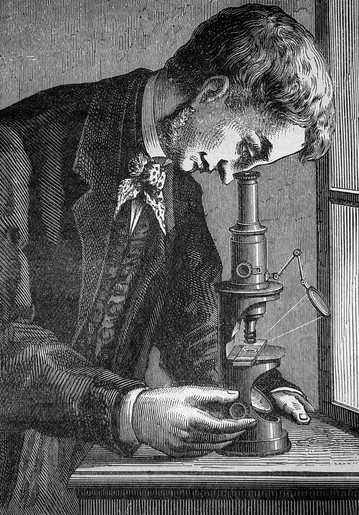
\includegraphics[width=\textwidth]{images/old_microscope.jpg}
		\end{subfigure}
		\begin{subfigure}{0.27\textwidth}
			\centering
			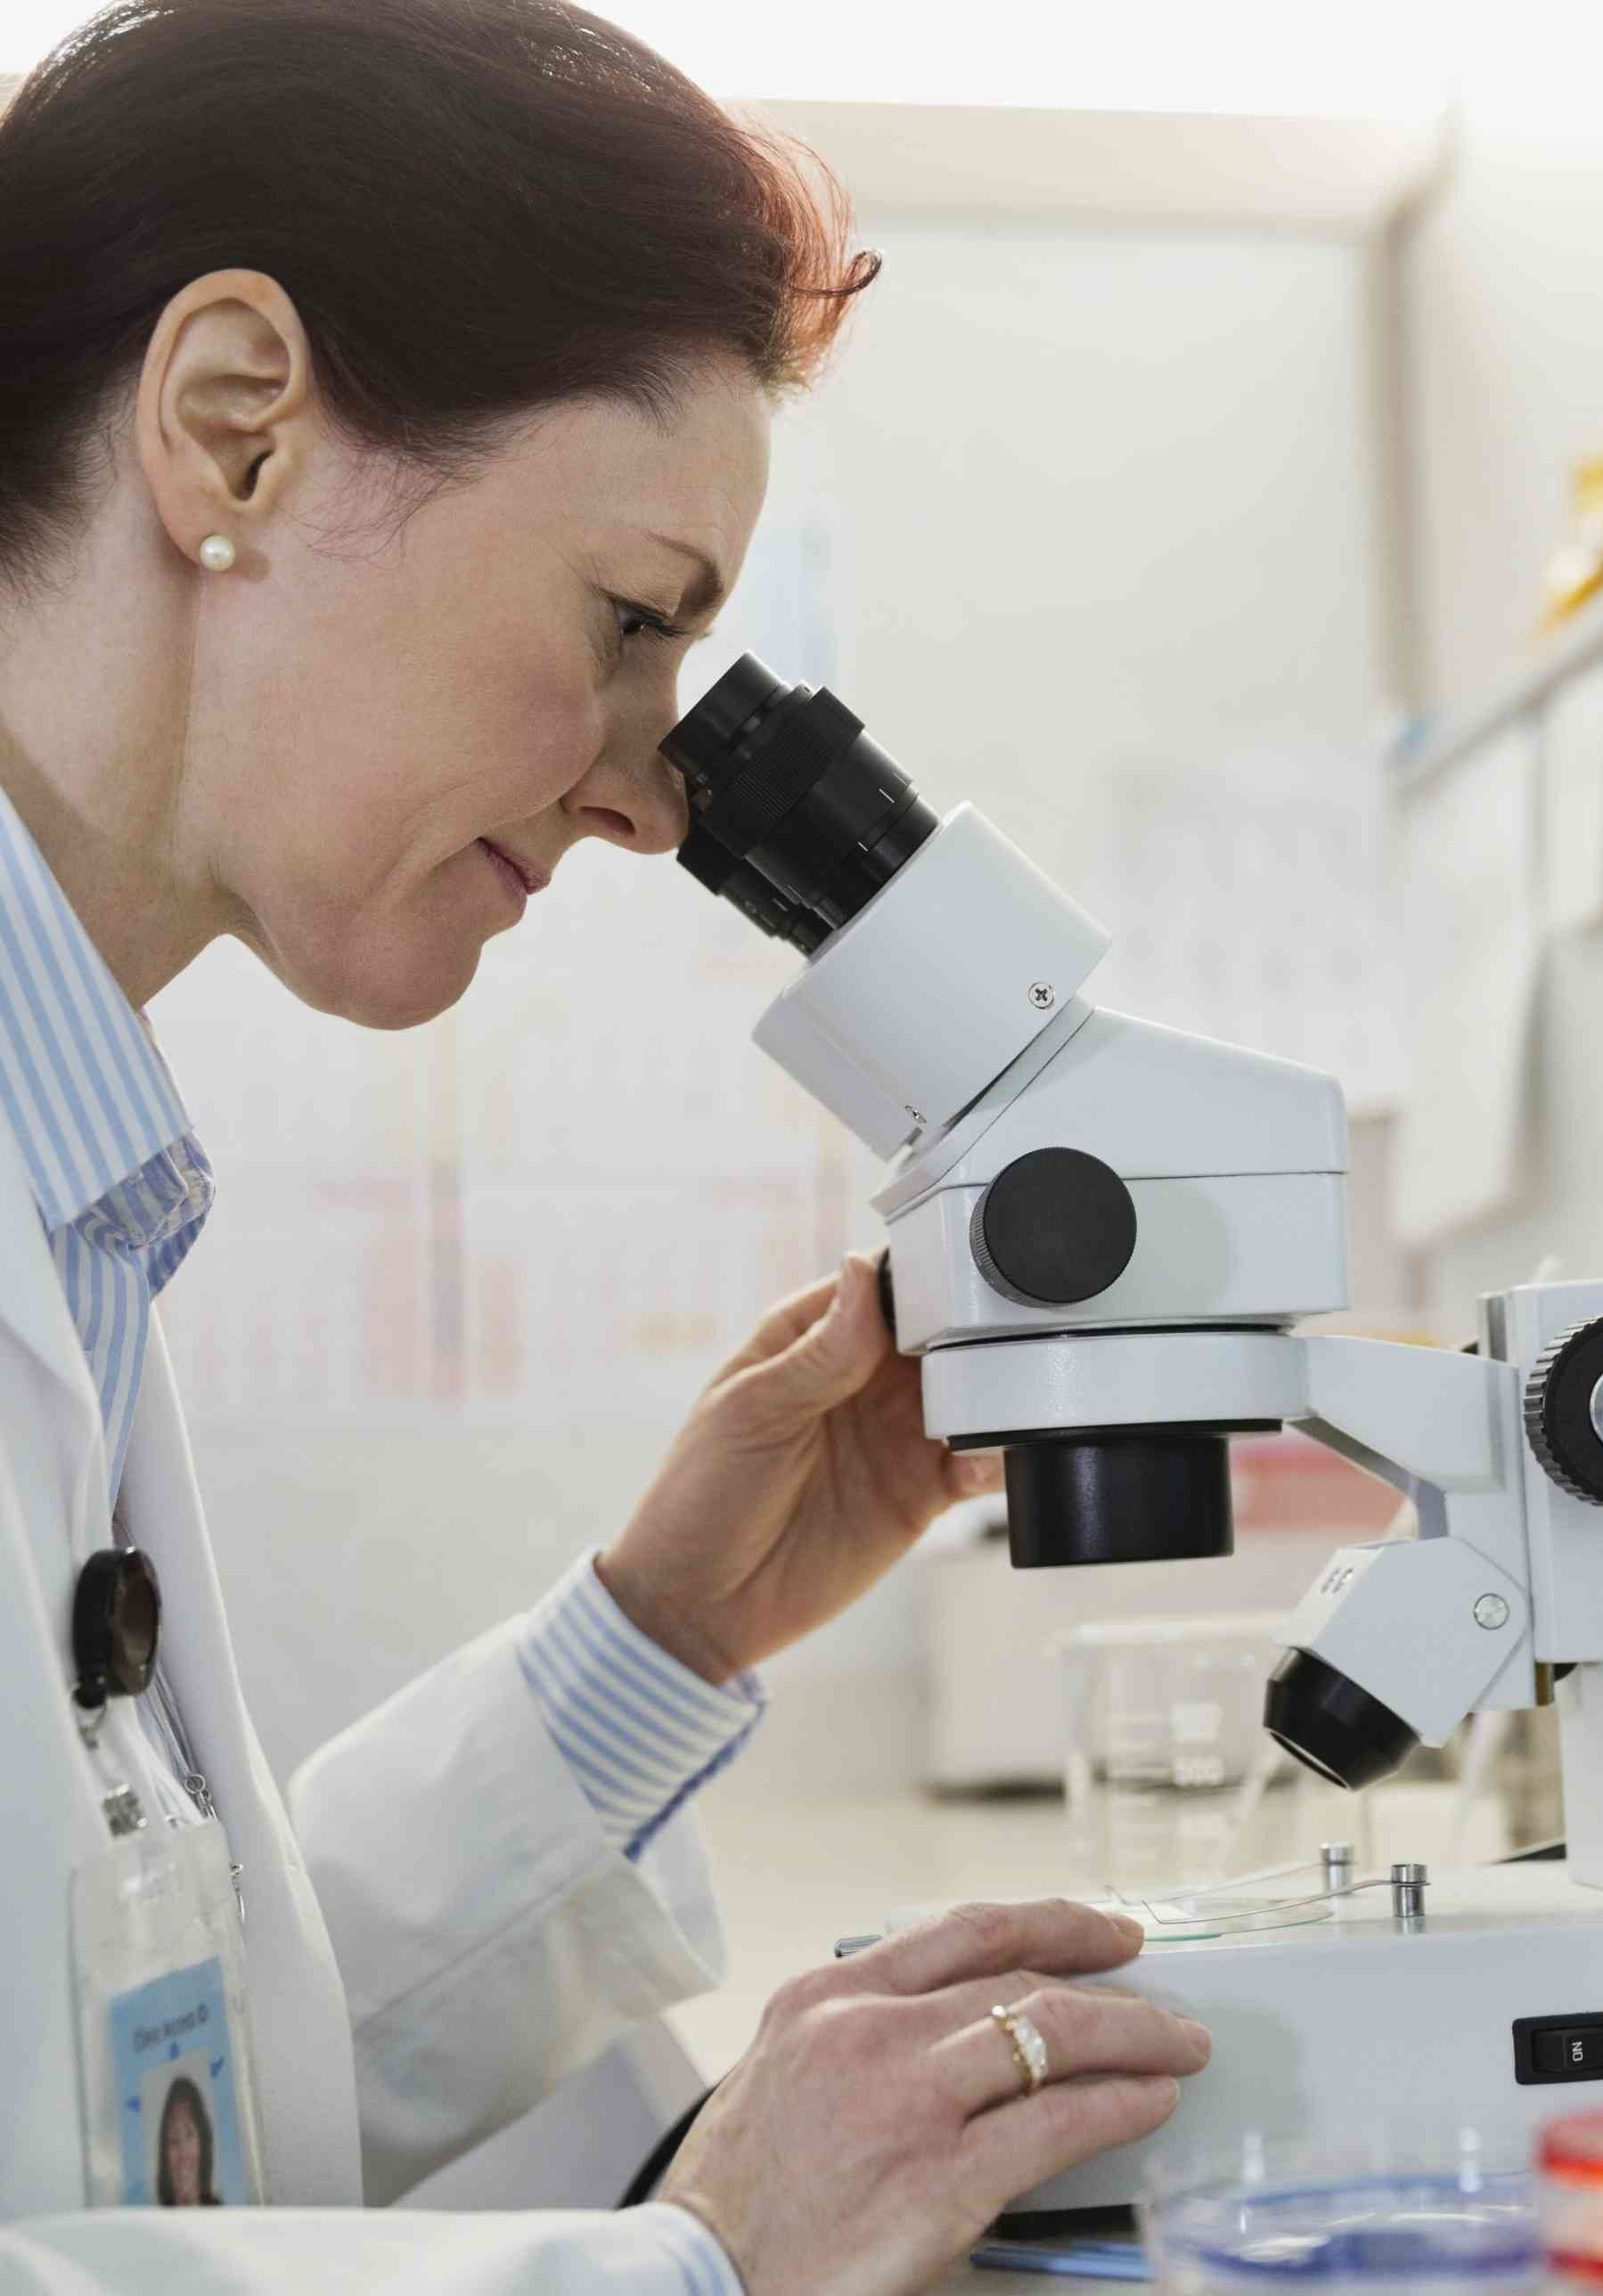
\includegraphics[width=\textwidth]{images/new_microscope.jpg}
		\end{subfigure}
		\begin{subfigure}{0.27\textwidth}
			\centering
			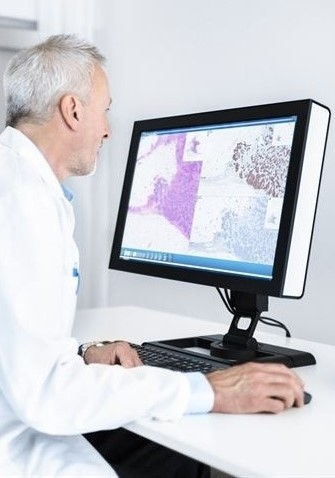
\includegraphics[width=\textwidth]{images/dpath_microscope.jpg}
		\end{subfigure}
	\end{figure}
	\begin{center}
	``\textit{Digital pathology incorporates the acquisition, management, sharing and \textbf{interpretation} of pathology information — including slides and data — in a digital environment}" 
	\end{center}
	\hfill
	{\tiny\textit{left:} institutions.ville-geneve.ch, \textit{center:} verywellhealth.com, \textit{right:} healthcare-in-europe.com}
\end{frame}
	
\begin{frame}{From the body to the computer}
	\vfill

	A pathology workflow: from a biopsy...
	\begin{figure}[h]
		\centering
		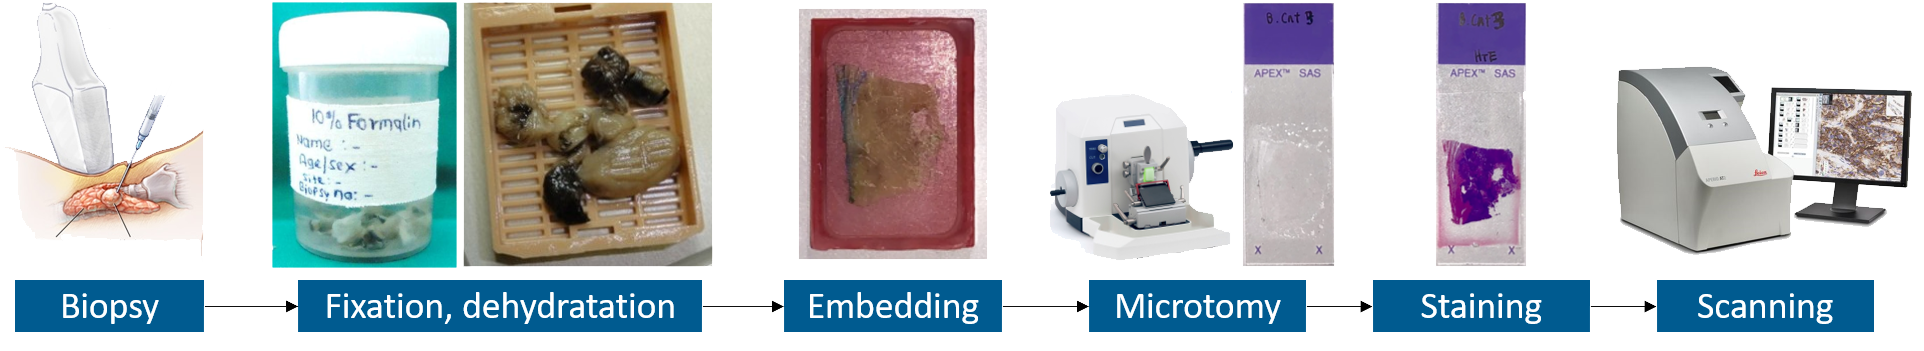
\includegraphics[width=\textwidth]{images/pathology_workflow.png}
	\end{figure}
	
	\vfill
	
	... to a whole-slide image and computer-assisted pathology.
	\begin{figure}
		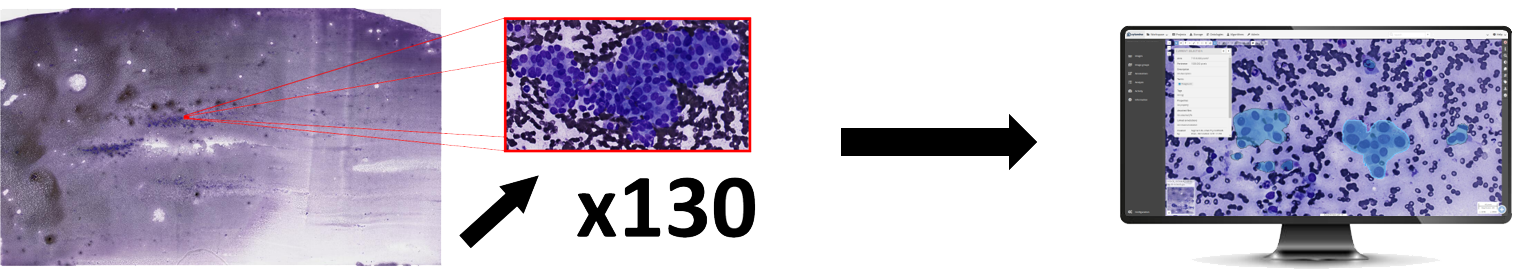
\includegraphics[width=\textwidth]{images/whole-slide-to-cap.png}
		\caption*{\small Left image: 163840 x 95744 pixels$^2$, 2.3 Gb.}
	\end{figure}
	
	\vfill
\end{frame}

\begin{frame}{Why computer-aided pathology}

\vfill

Some pathology analysis tasks are \textbf{tedious}, \textbf{time-consuming} and/or \textbf{costly}. 

Computational methods has the potential of making them faster, more reliable therefore \textbf{improving costs and patient outcome}. 

\vfill

\begin{figure}
	\begin{subfigure}{0.25\textwidth}
		\centering
		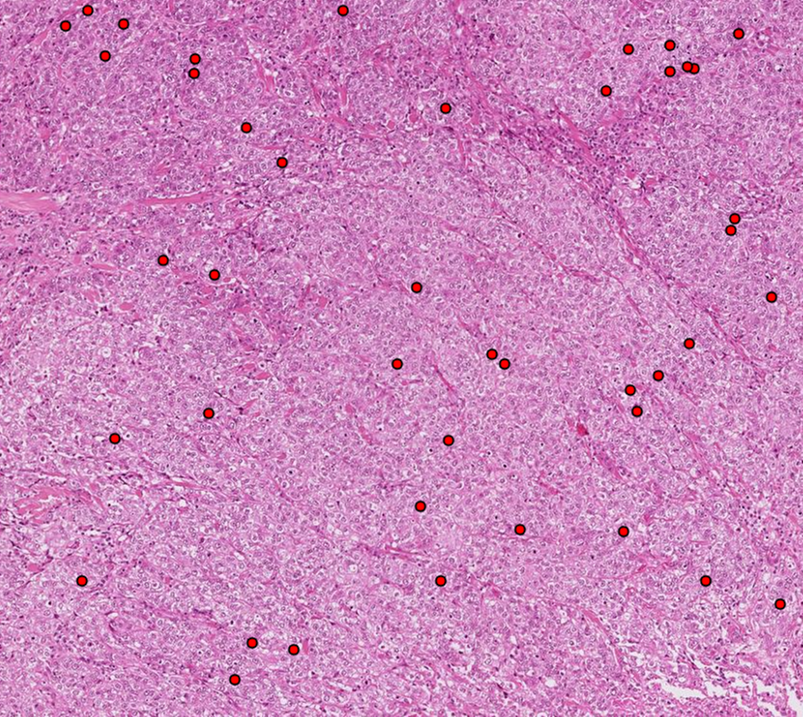
\includegraphics[width=\textwidth]{images/mitosis_zoomout.png}
		\caption{Counting}
	\end{subfigure}
	\begin{subfigure}{0.25\textwidth}
		\centering
		\vfill
		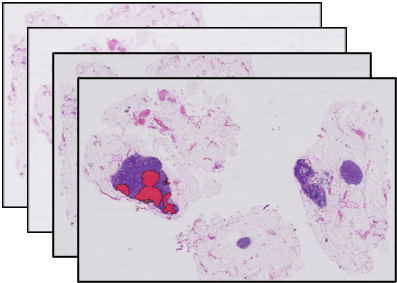
\includegraphics[width=\textwidth]{images/highdatavolume.png}
		\vfill
		\caption{Multi-slide analysis}
	\end{subfigure}
	\begin{subfigure}{0.25\textwidth}
		\centering
		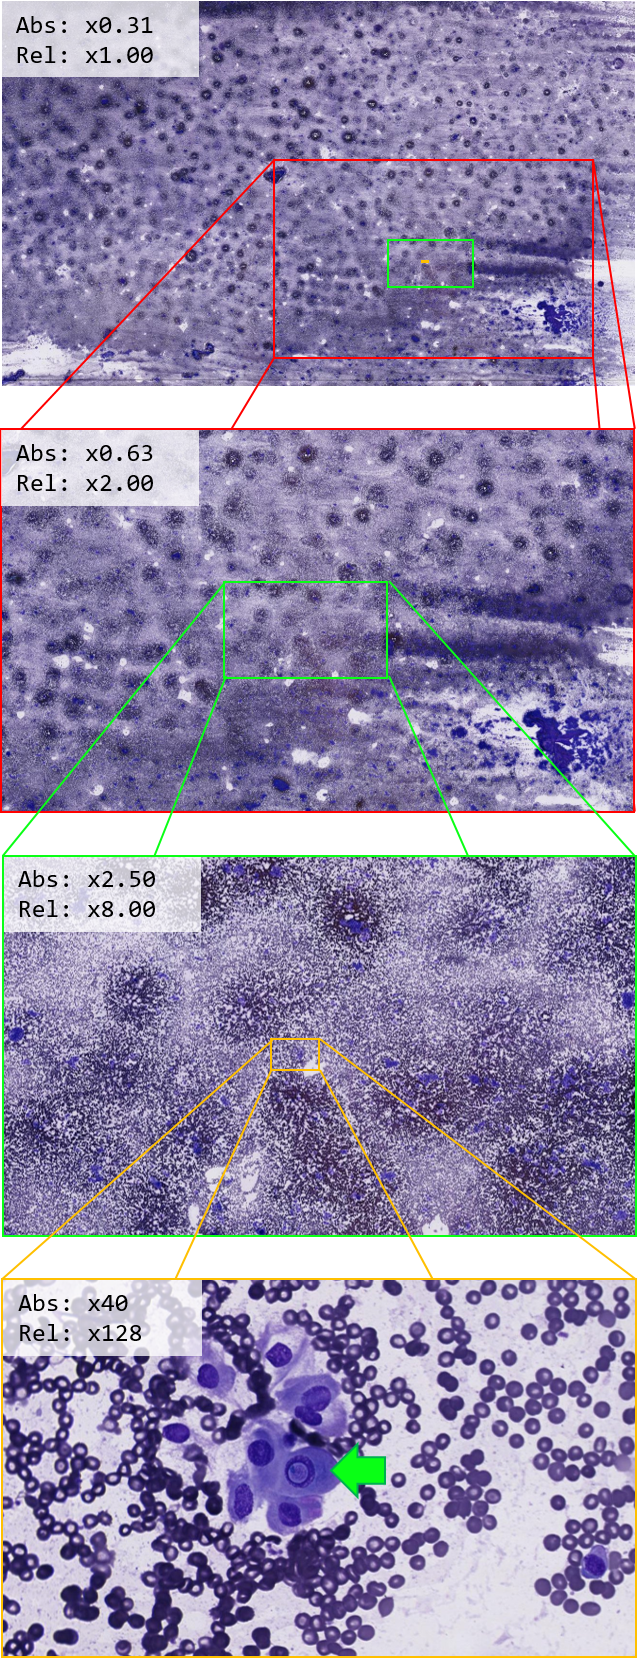
\includegraphics[height=0.2\textheight]{images/thyroid_needle_haystack.png}
		\caption{Needle in a haystack}
	\end{subfigure}
\end{figure}

\vfill
The field concerned with these methods is called \textbf{computational pathology}.

\vfill
\end{frame}

\begin{frame}{Computational pathology is challenging}
	Few of the challenges:
	\begin{itemize}
		\item {high variability}: content, staining, acquisition,...
		\item {data scarcity}: annotating data is expensive and tedious
		\item {big data}: up to millions of biological objects per multi-gigapixel image
	\end{itemize}
	\vfill
	\begin{center}
		\large
		\textbf{Machine learning methods} are excellent candidates for tackling these !
	\end{center}
\end{frame}

\begin{frame}{More on data scarcity}
Causes:
\begin{itemize}
	\item highly specialized annotators required
	\item simplification of the underlying medical problems
	\item privacy concerns
	\item deep learning methods are data hungry 
\end{itemize}

Consequences:
\begin{itemize}
	\item small datasets (compared to natural image domain)
	\item lack of variety on the problem targets 
	\item weakly- or sparsely-labeled datasets 
\end{itemize}
\end{frame}

\begin{frame}{Working around data scarcity}
Making more annotations within the same budget:
\begin{itemize}
	\item AI-assisted annotation
	\item appropriate UI/UX tools 
	\item citizen science/crowdsourcing
\end{itemize}

Using proper computational methods:
\begin{itemize}
	\item \textbf{transfer learning}
	\item \textbf{self-training}
	\item weakly-supervised learning
	\item self-supervised learning
\end{itemize}
\end{frame}


\section{Contributions}

\begin{frame}{Contributions}
	All contributions address digital patholog:
	\begin{itemize}
		\item Comparison of deep transfer learning strategies from ImageNet
		\item Multi-task pre-training of deep neural networks on pathology tasks
		\item Self-training for segmentation from sparsely-labeled data
	\end{itemize}
\end{frame}

\section{Transfer from ImageNet}
\subsection{Introduction}

\begin{frame}{Deep transfer learning: how to?}
	\begin{figure}
		\centering
		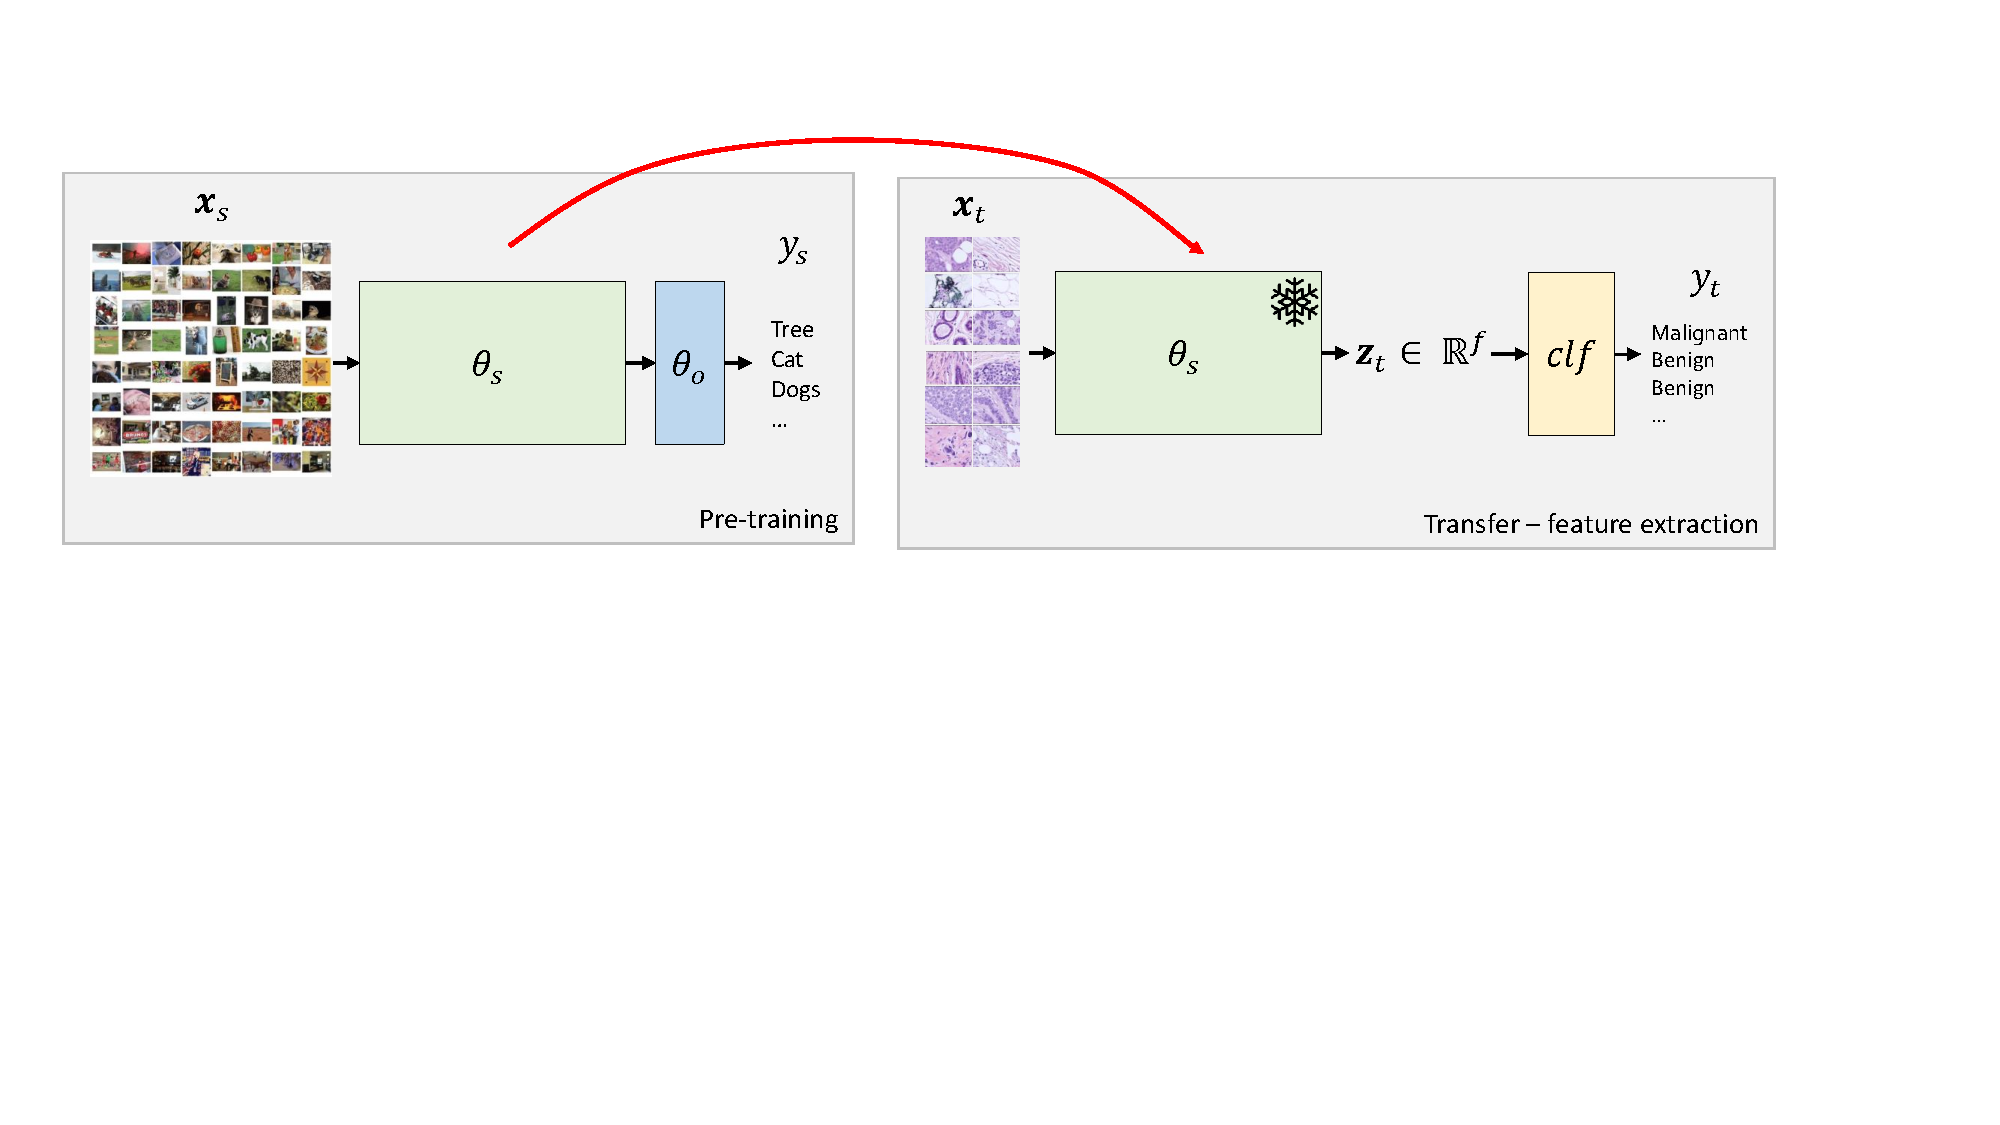
\includegraphics[width=0.9\textwidth]{images/transfer-fe.pdf}
		\caption*{Feature extraction}
	\end{figure}
	\begin{figure}
		\centering
		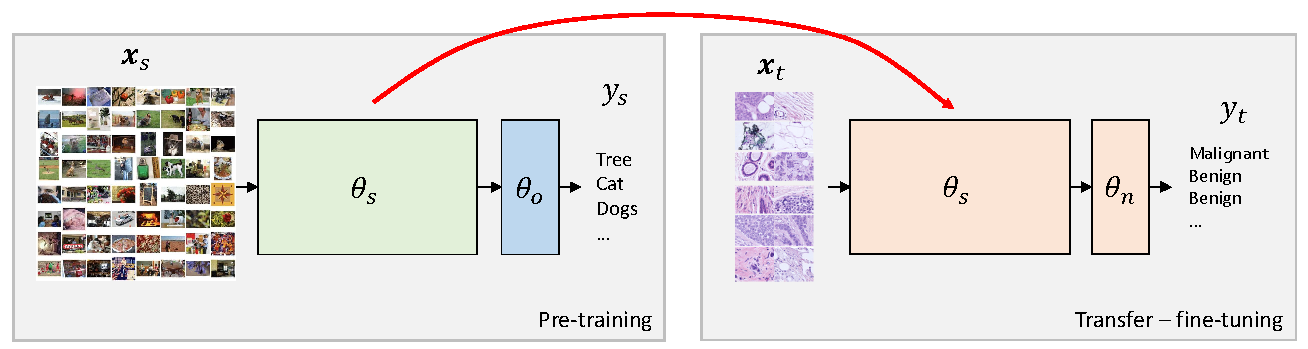
\includegraphics[width=0.9\textwidth]{images/transfer-ft.pdf}
		\caption*{Fine tuning}
	\end{figure}
\end{frame}

\begin{frame}{Our contribution}

\textbf{Goal}: devise \textbf{guidelines and best practices} for deep transfer learning in computational pathology

\vfill

\begin{itemize}
	\item {Fine-tuning \textit{vs.} feature extraction}: which one works better ? 
 	\item Which {pre-trained network} works better ? 
 	\item {Where to extract} features ? 
 	\item ...
\end{itemize} 

\vfill
We have carried out several experiments \textbf{with ImageNet} as source task:
\vfill
\begin{itemize}
	 \item \textbf{Feature extraction} vs. \textbf{fine-tuning}
	 \item \textbf{Networks}: ResNet50, DenseNet201, VGG16/19, InceptionResNetV2, \textit{etc}.
	 \item \textbf{Features classifiers}: SVM , extra-trees (ET), \textit{etc}.
	 \item Features extraction at {increasing depth}
	 \item Feature relevance evaluation
\end{itemize}
\end{frame}


\subsection{Data}
\begin{frame}{Datasets}
8 image classification datasets. 

\begin{table}
    \center 
    \footnotesize
    \begin{tabular}{|c|c|c|cc|}
        \hline
        \multirow{2}{*}{Dataset} & \multirow{2}{*}{Domain} & \multirow{2}{*}{Cls} & \multicolumn{2}{c|}{Total} \\
        \cline{4-5}
        & & & Images & Slides \\
        \hline
        Necrosis (N) & Histo & 2 & 882 & 13 \\ % ulg_lbtd2_chimio_necrose
        ProliferativePattern (P) & Cyto & 2 & 1857 & 36 \\ % patterns_no_aug
        CellInclusion (C) & Cyto & 2 & 3638 & 45 \\ % cells_no_aug
        MouseLba  (M) & Cyto & 8 & 4284 & 20 \\ % ulg_lbtd_lba
        HumanLba (H) & Cyto & 9 & 5420 & 64 \\ % ulb_anapath_lba
        Lung (L) & Histo & 10 & 6331 & 882 \\ % ulg_lbtd_tissus
        Breast (B) & Histo & 2 & 23032 & 34 \\ % ulg_lbtd2_chimio_necrose
        Glomeruli (G) & Histo & 2 & 29213 & 205 \\ % glomeruli_no_aug
        \hline
    \end{tabular}
\end{table}
\begin{figure}
    \center
    \begin{subfigure}{0.1\textwidth}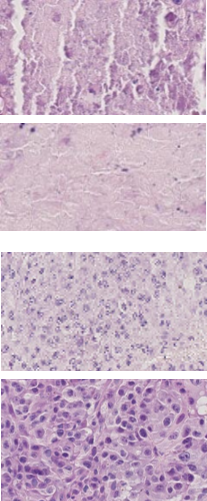
\includegraphics[scale=0.35]{images/illus_necrose.png}\end{subfigure}
    \begin{subfigure}{0.1\textwidth}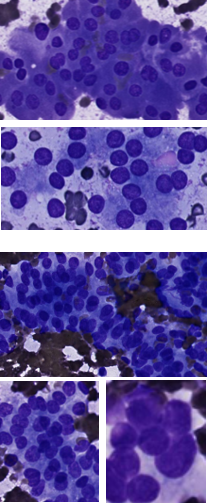
\includegraphics[scale=0.35]{images/illus_patterns.png}\end{subfigure}
    \begin{subfigure}{0.1\textwidth}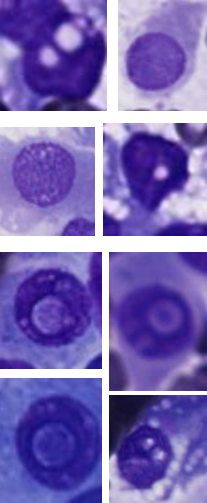
\includegraphics[scale=0.35]{images/illus_cells.png}\end{subfigure}
    \begin{subfigure}{0.1\textwidth}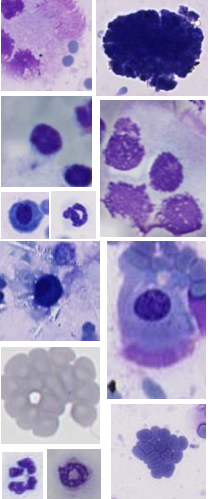
\includegraphics[scale=0.35]{images/illus_lbtd_lba.png}\end{subfigure}
    \begin{subfigure}{0.1\textwidth}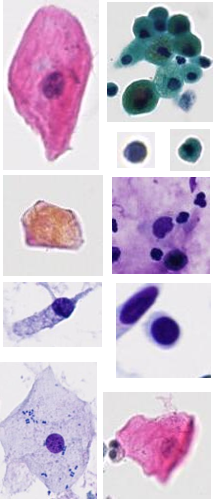
\includegraphics[scale=0.35]{images/illus_anapath.png}\end{subfigure}
    \begin{subfigure}{0.1\textwidth}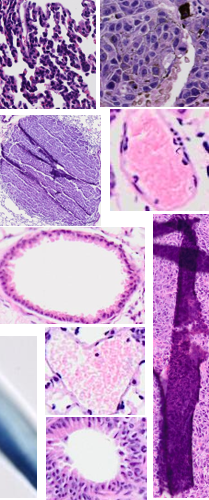
\includegraphics[scale=0.35]{images/illus_tissus.png}\end{subfigure}
    \begin{subfigure}{0.1\textwidth}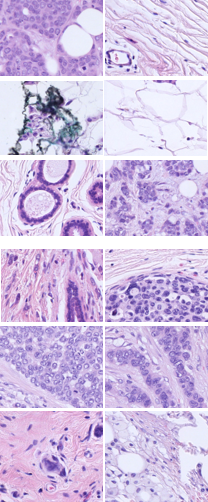
\includegraphics[scale=0.35]{images/illus_breast.png}\end{subfigure}
    \begin{subfigure}{0.1\textwidth}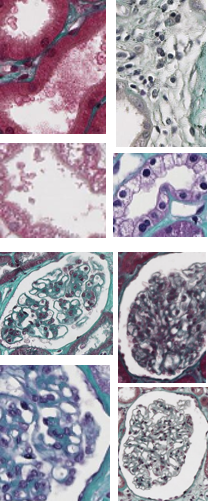
\includegraphics[scale=0.35]{images/illus_glomeruli.png}\end{subfigure}
\end{figure}

\end{frame}

\subsection{Experiments and results}
\begin{frame}{Results}
\framesubtitle{Fine-tuning is the best performing strategy}

\begin{center}
	{Fine-tuning} is often the best performing method \\
	... but {extracted features} are {close} on most problems and {less computationally expensive} !
\end{center}
\vfill
\begin{table}
	\center
	\tiny
	\begin{tabular}{l|ccccc|ccc}   
	  & \multicolumn{8}{c}{\textbf{Datasets}} \\
	  \hline 
	  \textbf{Strategy} & \textbf{Cell} & \textbf{Prolif} & \textbf{Glom} & \textbf{Necro} & \textbf{Breast} & \textbf{Mouse} & \textbf{Lung} & \textbf{Human} \\
	  \hline
	  Baseline (ET-FL)      & {\color{grey}0.9250} & {\color{grey}0.8268} & {\color{grey}0.9551} & {\color{grey}0.9805}	& {\color{grey}0.9345} & {\color{grey}0.7568} & {\color{grey}0.8547} & {\color{grey}0.6960} \\
	  Last layer    & {\color{grey}0.9822} & {\color{grey}0.8893} & {\color{grey}0.9938} & \textit{0.9982} & {\color{grey}0.9603} & {\color{grey}0.7996} & {\color{grey}0.9133}	& {\color{grey}0.7820} \\
	  Feat. select.	& {\color{grey}0.9676}	& {\color{grey}0.8861}	& {\color{grey}0.9843}	& \textbf{0.9994}	& {\color{grey}0.9597}	& {\color{grey}0.7438}	& {\color{grey}0.8941}	& {\color{grey}0.7703} \\
	  Merg. networks	& \textit{0.9897}	& \textbf{0.8984}	& {\color{grey}0.9948}	& {\color{grey}0.9864}	& {\color{grey}0.9549}	& \textit{0.8169}	& {\color{grey}0.9155}	& {\color{grey}0.7928} \\
	  Merg. layers	& {\color{grey}0.9808}	& {\color{grey}0.8906}	& {\color{grey}0.9944}	& {\color{grey}0.9964}	& {\color{grey}0.9639}	& {\color{grey}0.7941}	& {\color{grey}0.9268}	& {\color{grey}0.7977} \\
	  Inner ResNet	& {\color{grey}0.9748}	& \textit{0.8959}	& {\color{grey}0.9949}	& {\color{grey}0.9964}	& {\color{grey}0.9664}	& {\color{grey}0.8131}	& \textit{0.9291}	& \textit{0.8113} \\
	  Inner DenseNet	& {\color{grey}0.9862}	& \textbf{0.8984}	& \textit{0.9962}	& {\color{grey}0.9917}	& {\color{grey}0.9699}	& {\color{grey}0.8012}	& {\color{grey}0.9268}	& {\color{grey}0.7967} \\
	  Inner IncResV2	& {\color{grey}0.9873}	& {\color{grey}0.8948}	& \textit{0.9962}	& \textit{0.9982}	& \textit{0.9720}	& {\color{grey}0.8137}	& {\color{grey}0.9234}	& {\color{grey}0.7713} \\
%       Inner IncV3		& {\color{grey}0.9836}	& {\color{grey}0.8899}	& {\color{grey}0.9951}	& {\color{grey}0.9964}	& {\color{grey}0.9731}	& {\color{grey}0.8104}	& {\color{grey}0.9201}	& {\color{grey}0.7507} \\
	   {Fine-tuning}		& \textbf{0.9926}	& {\color{grey}0.8797}	& \textbf{0.9977}	& {\color{grey}0.9970}	& \textbf{0.9873}	& \textbf{0.8727}	& \textbf{0.9405}	& \textbf{0.8641} \\
%%      \hline
%%      \textbf{Best} & 0.9926 & 0.8984 & 0.9977 & 0.9994 & 0.9873 & 0.8727 & 0.9405 & 0.8641 \\
	  \hline
	  \textbf{Metric} & \multicolumn{5}{c|}{Roc AUC} & \multicolumn{3}{c}{Accuracy (multi-class)} \\
	\end{tabular}
	\caption{\footnotesize Best in \textbf{bold}, second best in \textit{italic}}
\end{table}
\end{frame}


\begin{frame}{Results}
\framesubtitle{When working with extracted features, use some inner layer features}
	\vfill	
	\begin{figure}
		\center
		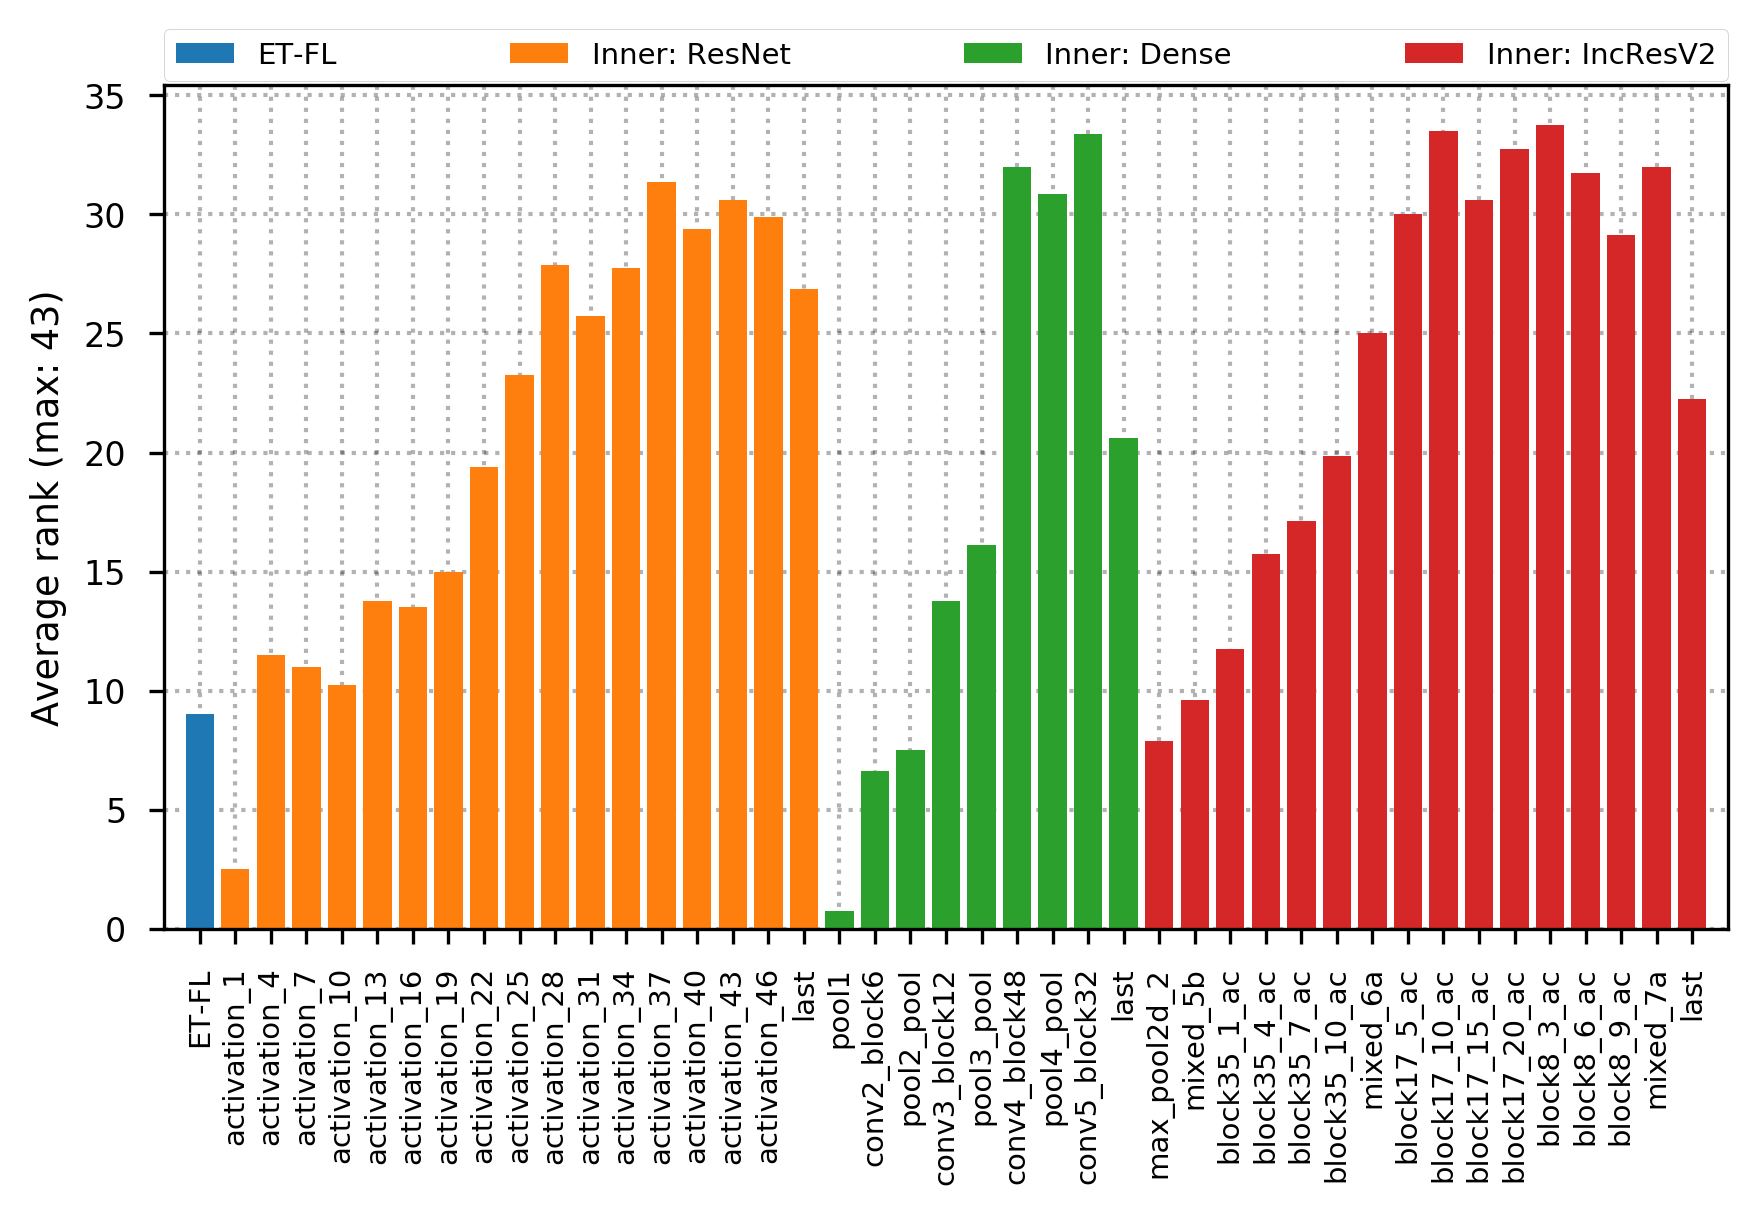
\includegraphics[scale=0.7]{images/all_per_layer_hori_bars.png}
	\end{figure}
	\vfill
\end{frame}


\begin{frame}{Results}
\framesubtitle{More recent networks like DenseNet or ResNet work better}
\begin{figure}
	\center
	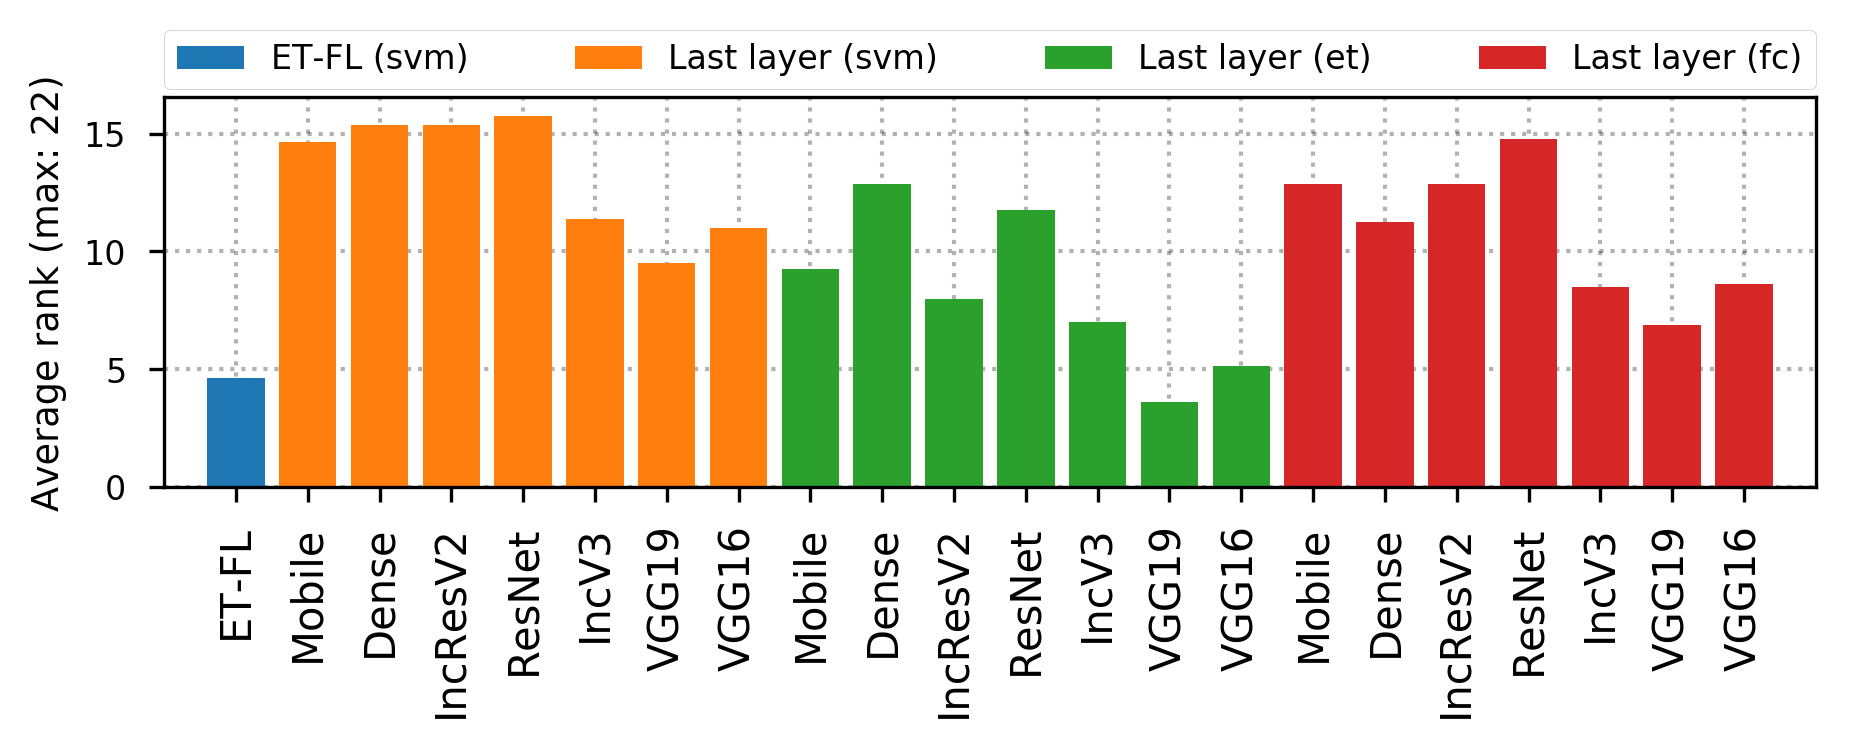
\includegraphics[scale=0.65]{images/last_baseline_bars.png}
\end{figure}

{\footnotesize
	\textbf{See also:} \fullcite{kornblith2019better}
}
\end{frame}

\begin{frame}{Conclusion}
	\vfill
	Main {takeaways}:
	\vfill
	\begin{itemize}
		\item {Fine tuning} is the best performing method
		\item {Features extraction} often close to fine-tuning and less computationally expensive
		\item Prefer {inner layers feature extraction} to last layers feature extraction
		\item Use {more recent networks} such as DenseNet and ResNet
	\end{itemize}
	\vfill
	
\end{frame}

\section{Transfer from pathology data}

\begin{frame}

\end{frame}

\section{Self-training}
\begin{frame}{An imperfect cytology dataset: thyroid nodules}
	
\end{frame}

\begin{frame}{Binary segmentation with a sparse dataset ?}
	\vfill
	\begin{center}
		Let's generate pseudo-labels for unlabelled pixels before training !
	\end{center}
	\vfill
	\begin{center}
	  How ? With a \textbf{self-training} algorithm !
	\end{center}
	\vfill
\end{frame}

\subsection{Problem settings}
\begin{frame}{Problem settings}
\framesubtitle{A sparsely-labelled dataset}
	\begin{columns}[t]
		\begin{ccolumn}{0.48\textwidth}{$\mathcal{D}_l$ - exhaustively-labelled set}
			
			\begin{figure}
				\center
				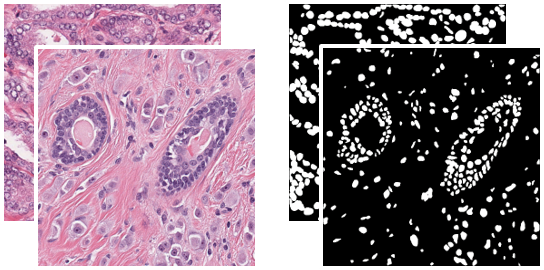
\includegraphics[width=\textwidth]{images/exhaustive_set.png}
				\caption*{$n_l$ images and masks. All pixels have a 0 (background) or 1 (foreground) label.}
			\end{figure}
		\end{ccolumn}
		% --------------------------
		\begin{ccolumn}{0.48\textwidth}{$\mathcal{D}_s$ - sparsely-labelled set}
			\begin{figure}
				\center
				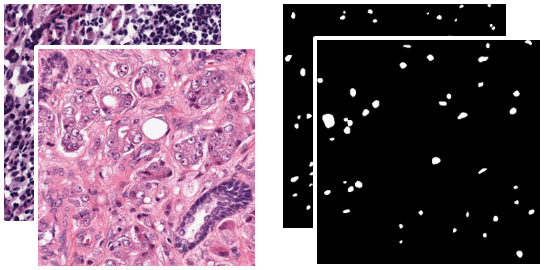
\includegraphics[width=\textwidth]{images/sparse_set.png}
				\caption*{$n_s$ images and masks. Unlabelled pixels have label 0 (background) and labelled pixels are exclusively foreground.}
			\end{figure}
		\end{ccolumn}
	\end{columns}
\end{frame}

\begin{frame}{Problem settings}
\framesubtitle{A segmentation architecture}
	\vfill
	A downscaled UNet \cite{ronneberger2015unet} architecture: reduce the number of parameters by a factor 8. 
	\vfill
	\begin{figure}
		\centering
		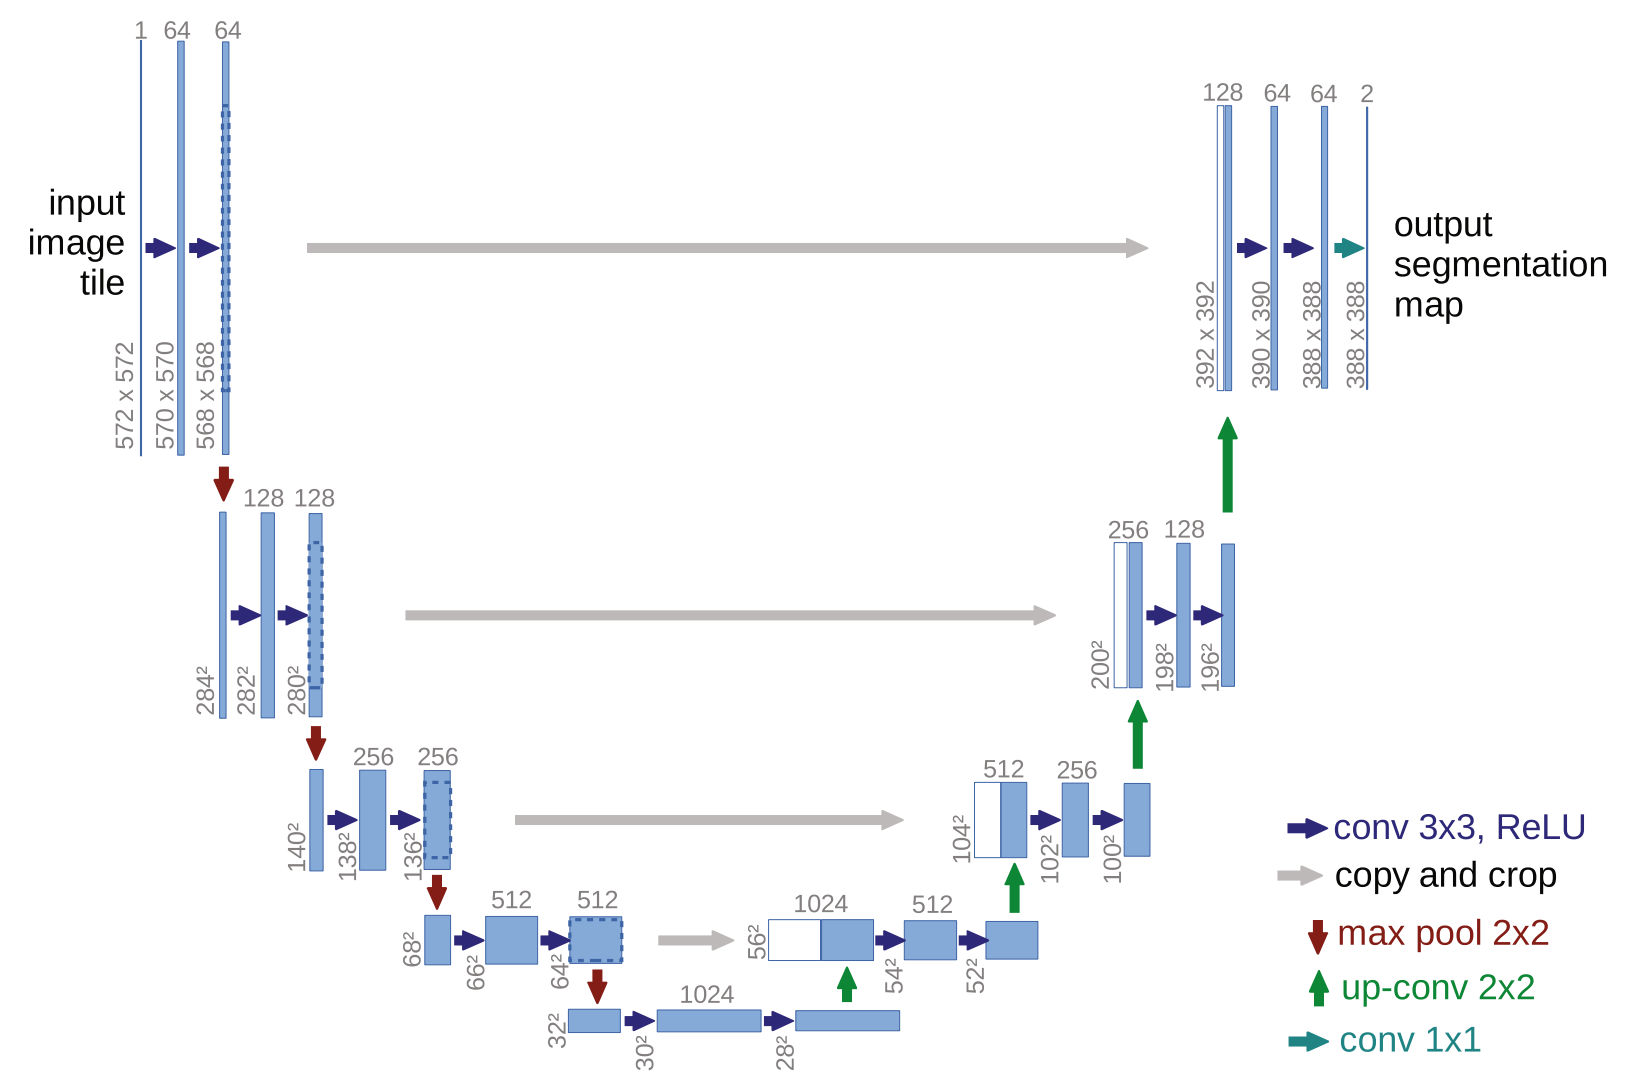
\includegraphics[height=0.7\textheight]{images/unet.png}
	\end{figure}
	\vfill
\end{frame}

\subsection{Our algorithm}
\begin{frame}{Our self-training algorithm}
	\centering
	\begin{figure}
		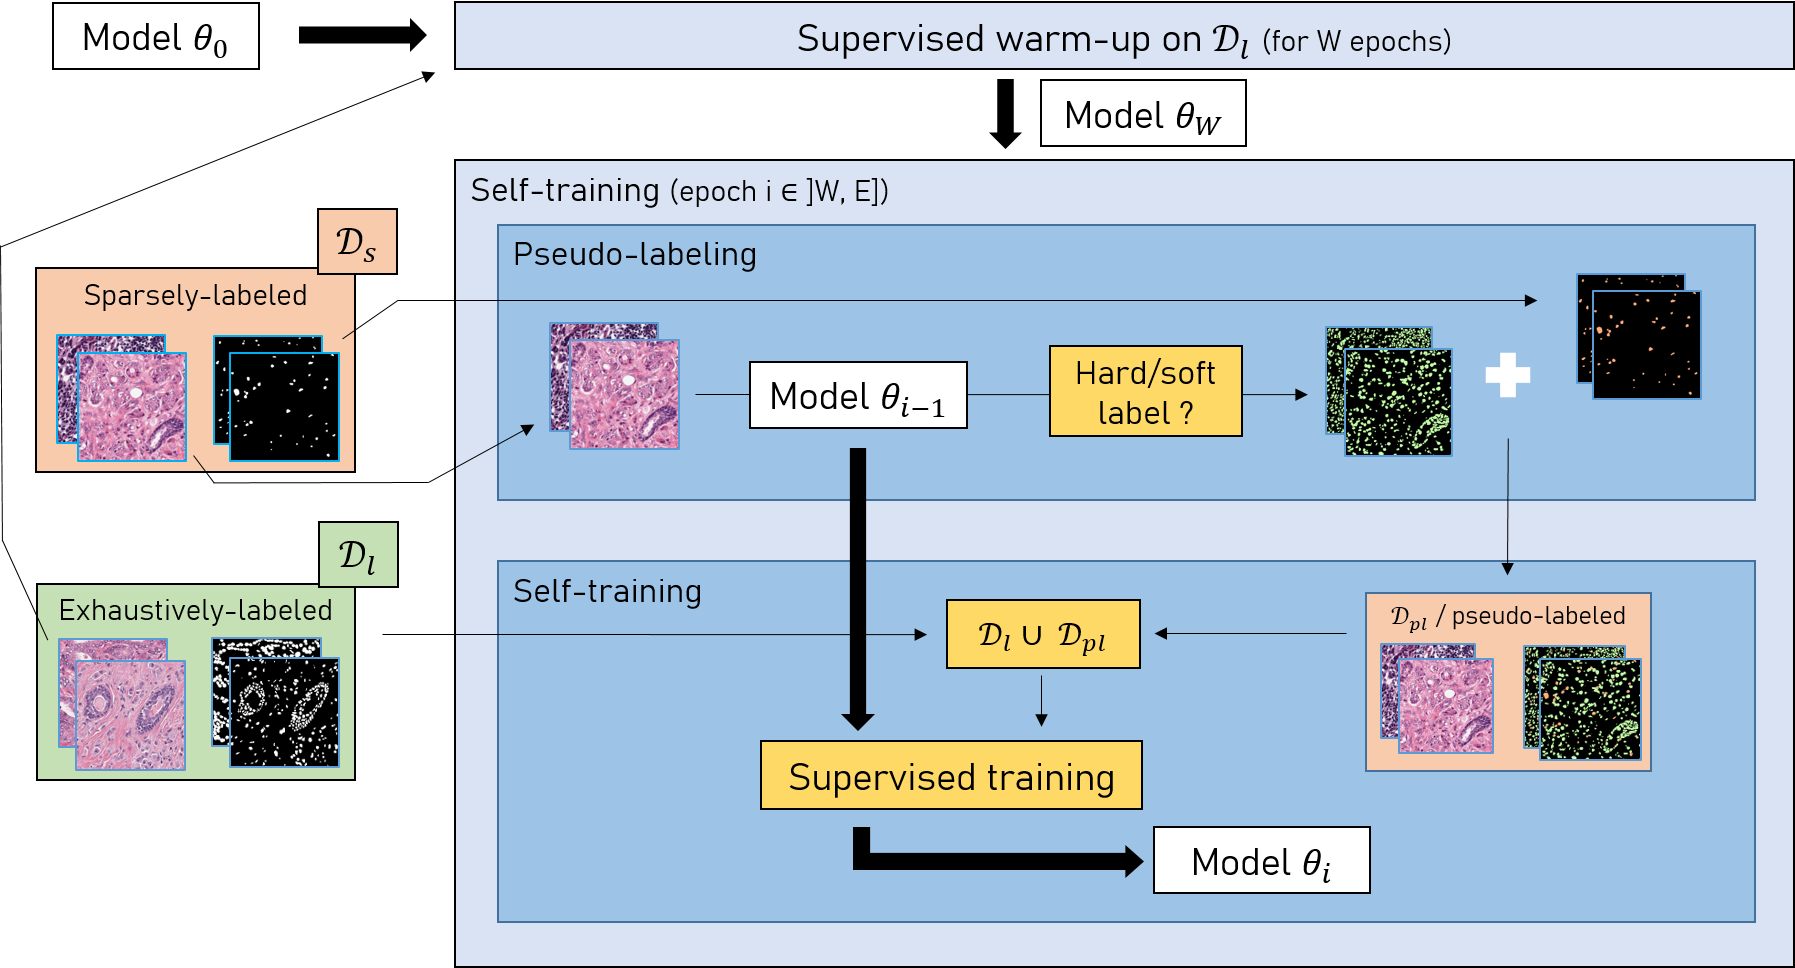
\includegraphics[width=\textwidth]{images/selftrain-algo.png}
	\end{figure}
\end{frame}

\subsection{Experiments}
\begin{frame}{Experiments}
\framesubtitle{3 public datasets}
	\centering
	\begin{columns}
		\begin{ccolumn}{0.30\textwidth}{MoNuSeg \cite{kumar2019multi}}
			\centering 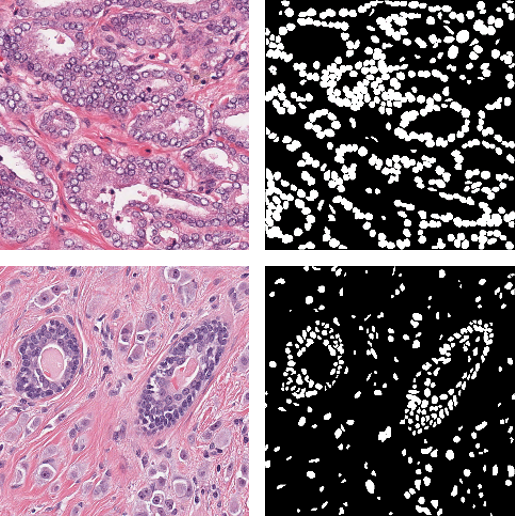
\includegraphics[width=\textwidth]{images/monuseg_rep.png}
		\end{ccolumn}
		% --------------------------
		\begin{ccolumn}{0.30\textwidth}{SegPC \cite{gupta2021segpc}}
			\centering 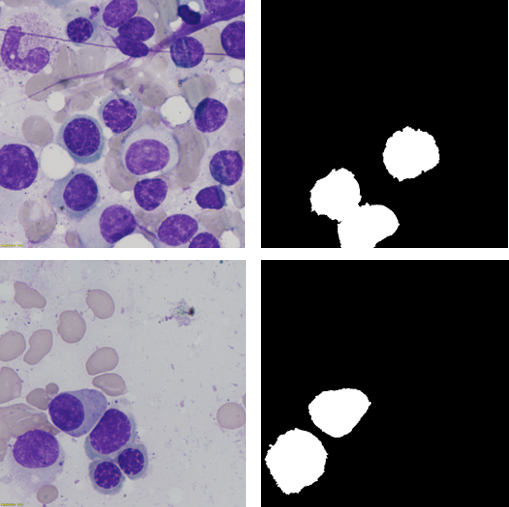
\includegraphics[width=\textwidth]{images/segpc_rep.png}
		\end{ccolumn}
		% --------------------------
		\begin{ccolumn}{0.30\textwidth}{GlaS \cite{sirinukunwattana2017gland}}
			\centering 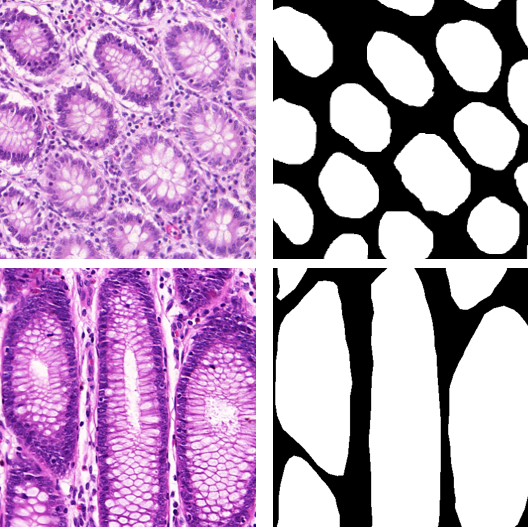
\includegraphics[width=\textwidth]{images/glas_rep.png}
		\end{ccolumn}
	\end{columns}
	\vfill
	Sparsity is simulated by randomly removing $\rho \%$ of annotations in $n_s$ images.
	\vfill
\end{frame}

\begin{frame}{Experiments}
\framesubtitle{3 public baselines}
	\vfill
	\begin{columns}[t]
		\begin{ccolumn}{0.30\textwidth}{(1) $|\mathcal{D}_s| = 0$ }
			\begin{figure} \centering 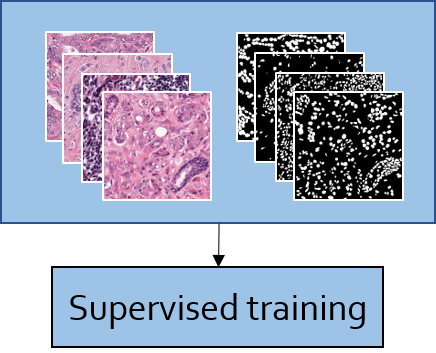
\includegraphics[height=0.3\textheight]{images/baseline1.png} \end{figure}%
\vspace{-0.8cm}
\begin{flushright}{\tiny (orignal dataset)}\end{flushright}
		\end{ccolumn}
		\begin{ccolumn}{0.30\textwidth}{(2) $\mathcal{D}_l$ only}
			\begin{figure} \centering 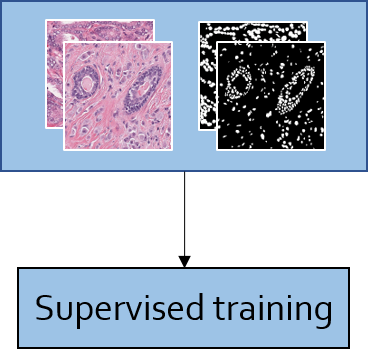
\includegraphics[height=0.3\textheight]{images/baseline2.png} \end{figure}
		\end{ccolumn}
		\begin{ccolumn}{0.30\textwidth}{(3) $\mathcal{D}_l \cup \mathcal{D}_s$}
			\begin{figure} \centering 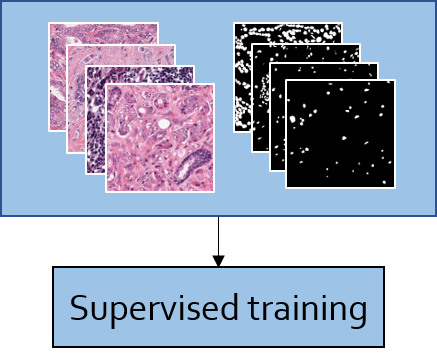
\includegraphics[height=0.3\textheight]{images/baseline3.png} \end{figure}%
\vspace{-0.5cm}
\begin{raggedright}{\tiny (unlab. pixels assigned to background)}\end{raggedright}%
		\end{ccolumn}
	\end{columns}
	\vfill
	\begin{center}
		To be considered of interest, our method should be as close as possible to (1) (upper bound) and outperform baselines (2) and (3).
	\end{center}
	\vfill
\end{frame}

\subsection{Results}
\begin{frame}{Results}
\framesubtitle{Hard vs. soft labeling}
\end{frame}

\begin{frame}{Results}
\framesubtitle{Self-training at fixed $n_l$}
\end{frame}

\begin{frame}{Results}
\framesubtitle{Label sparsely or exhaustively ?}
\end{frame}

\begin{frame}{Results}
\framesubtitle{Tuning the segmentation threshold}
\end{frame}

\begin{frame}{Results}
\framesubtitle{An actually sparse dataset: Thyroid FNAB}
% present the application of the model
\end{frame}

\begin{frame}{Self-training: conclusion}
\end{frame}

\begin{frame}{Using the model for Thyroid FNAB}
	% present the results 
\end{frame}

%\begin{frame}{Deep learning}
%\vspace*{-0.5cm}
%\begin{columns}
%%
%   \begin{ccolumn}{0.48\textwidth}{blue}{Training from scratch}
%   		Initialize weights randomly and train as usual.
%        \begin{itemize}
%			\item[$-$] Needs lots of data
%			\item[$-$] Needs much computing resources 
%		\end{itemize}
%    \end{ccolumn}
%
%
%\end{columns}
%\begin{columns}
%
%	\begin{ccolumn}{0.48\textwidth}   {red}{Off-the-shelf}
%		Use pre-trained weight, then use features off-the-shelf.
%		\begin{itemize}
%			\item[$+$] Needs less data then training from scratch
%			\item[$+$] Needs less computing resources 
%		\end{itemize}
%	\end{ccolumn}
%
%
%
%	\begin{ccolumn}{0.48\textwidth}{green}{Fine-tuning}
%		Initialize with pre-trained weigths, and train for few epochs.
%		\begin{itemize}
%			\item[$+$] Needs less data than training from scratch
%			\item[$-$] Needs much computing resources 
%		\end{itemize}
%	\end{ccolumn}
%
%\end{columns}	
%
%\end{frame}
%\begin{frame}{Deep transfer learning: how to ?}
%\textbf{Aim}: evaluate which \textbf{deep transfer learning} strategy yields best results using the 8 datasets.
%
%\begin{itemize}
%	\item Deep learning works well with images 
%	\item Transfer learning usually requires less data and computing resources {\color{red} (cite)}
%	\item DTL has been applied to biomedical problems since 2015 {\color{red} (cite)}
%\end{itemize} 
%
%But... \textbf{few people have actually studied how DTL should be applied} !
%
%\begin{itemize}
%	\item most publications use "old" networks (AlexNet, VGGs, GoogLeNet,...)
%	\item studies which do are often too small scale to draw general conclusions 
%\end{itemize}
%\end{frame}
%
%\begin{frame}{Framework}
%\begin{figure}
%	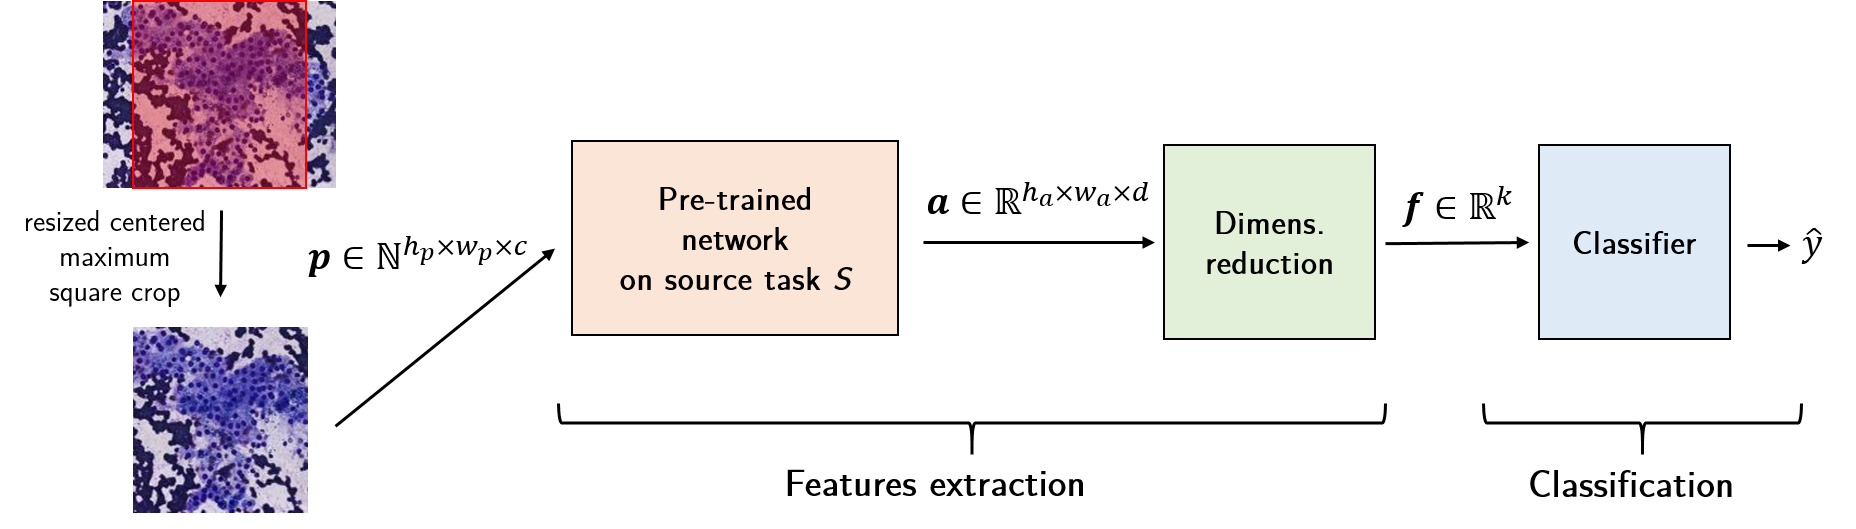
\includegraphics[scale=0.35]{images/offtheshelf_schema.png}
%\end{figure}
%\end{frame}
%
%\begin{frame}{Transfer strategies}
%\begin{columns}
%
%\begin{column}{0.31\textwidth} 
%	\begin{orangebox}{Last layer features}
%		
%	\end{orangebox}
%\end{column}
%
%\begin{column}{0.31\textwidth} 
%	\begin{greenbox}{Feature selection}
%		
%	\end{greenbox}
%\end{column}
%
%\begin{column}{0.31\textwidth}
%	\begin{redbox}{Merging models}
%		
%	\end{redbox} 
%\end{column}
%
%\end{columns}
%
%\begin{columns}
%
%\begin{column}{0.31\textwidth} 
%	\begin{purplebox}{Merging networks}
%		
%	\end{purplebox}
%\end{column}
%
%\begin{column}{0.31\textwidth} 
%	\begin{brownbox}{Fine-tuning}
%		
%	\end{brownbox}
%\end{column}
%
%\begin{colorbox}{0.31\textwidth}{bluebox}{Inner layers}
%\end{colorbox}
%
%\end{columns}
%\end{frame}
\end{document}
